\section{\ToolP view-aware optimization}
\label{sec:opt}
%\shan{Are we not doing incremental loading any more?}
%\cong{``\Tool optimization'' sounds a bit confusing (optimization to static analysis?). maybe ``Suggesting code change''?}\shan{I changed this and last section titles. How about now?}\cong{looks good! :)}


\Tool suggests three categories of view-changing code refactoring
to improve page-load time:

%\Tool categorizes view-changing performance optimization into three categories:
%, ranging from less to more changes to the view of a web application:
\begin{enumerate}
    \item Display the same contents in a different style, such as pagination and asynchronous loading.
    \item Display the same contents but with a different accuracy.
    \item Remove a subset of contents from display.
\end{enumerate}

These code refactorings can be applied for different types of HTML tags, and complement each other. 

\ToolP code refactoring works independently from \ToolP cost estimator. As we will see in Section \ref{sec:ide}, \ToolP interface will contain both features and help developers make informed refactoring decisions.\shan{How about this?}


% This section explains how \Tool automatically detects the opportunities
% and generates the code changes of the above three categories of optimization.
% Since these optimizations all improve performance with certain
% cost of functionality, \Tool will offer them in an interactive development environment as we will
% present in Section \ref{sec:ide}, instead of through transparent 
% code changes.

\subsection{Display-style change: pagination}
\label{sec:pagi}

Many web pages are designed to display {\it all} database records satisfying
certain conditions. When the database size grows, such pages will take an increasingly 
more time to load, and eventually become unresponsive.

A widely used solution to this problem, called {\it pagination}, is to display only a fixed number 
of records in a page and allow users to navigate to other pages for more records.

% \iffalse
% For example, Diaspora is a popular social network application \cite{diaspora}. 
% %Its {\tt contacts/index} page used to list {\it all} the contacts of a user, 
% One page from this application used to list {\it all} the contacts of a user,
% which led to slow page-loading time complained by users with many contacts. 
% Later on, in one issue report~\cite{diaspora5335}
% %Diaspora-5335~\cite{diaspora5335}, 
% developers solved this performance problem
% by showing contacts page by page, with 25 contacts a page. \shan{quantitative time information
% would help}
% \fi

Although pagination is widely used in practice, there are still many cases where it is not used --- 14 out of 140 real-world performance
issues sampled by a previous study \cite{yang:icse18:hloop} are due to lack of pagination
--- either because developers are unaware of pagination, or because they did not anticipate the data size will become a
performance problem. Therefore, we design \ToolP to automatically identify
pagination opportunities and conduct corresponding refactoring 
for developers. \alvin{isn't this what we do? last sentence makes it sound like this is future work}

\subsubsection{Identifying opportunities}


\begin{figure}
    \centering
    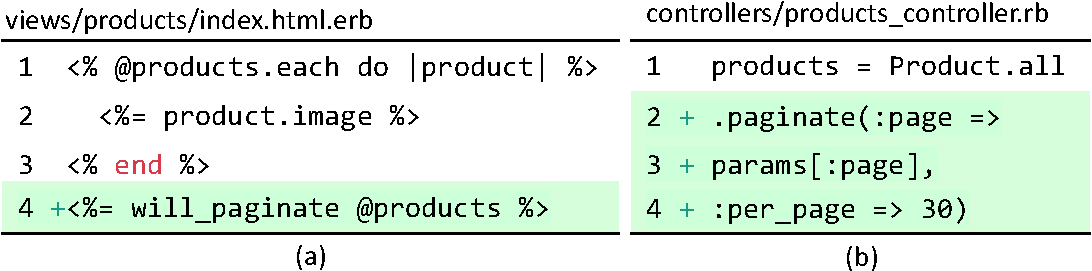
\includegraphics[width=\columnwidth]{panorama-figs//paginate.pdf}
    %\vspace{0.05in}
    \caption{Refactoring so that the paginated page displays 30 items at a time rather than the full list}
    \label{fig:pagi}
     \vspace{-0.2in}
\end{figure}

To identify these opportunities, \Tool checks each loop in the program for: (1) whether the loop iterates through the result of an unbounded query;
and (2) whether each loop iteration leads to some content being rendered in an HTML tag.
If a loop passes both checks, the corresponding HTML tag will be reported as a pagination candidate.

For the first check, \Tool locates the array variable that a loop iterates through, like {\tt @products} in
the loop shown in the left column of Figure \ref{fig:pagi}, and then
checks the data-flow edges in ADG to determine 
whether this variable is produced by an unbounded database query, as defined in Section \ref{sec:profile_static}.
For example, the ADG would show that {\tt @products} is the result of {\tt Product.all} on
Line~1 of in Figure~\ref{fig:pagi}b, and {\tt Product.all} will be translated to
an unbounded database query 
%which takes 1000ms \cong{what is 1000ms?}
at run time.

For the second check, \Tool searches for an ADG node $n_v$ that is associated with an HTML tag and an
{\tt is\_rendered} property inside the loop body (how to compute {\tt is\_rendered} is introduced in Sec. \ref{sec:annotateview}). If $n_v$ is found, like Line 2
in  Figure \ref{fig:pagi}a,
%(in both lines, the {\tt \%=} prefix 
%indicates that the Ruby variable following the prefix will be rendered),
the HTML tag associated with $n_v$ is identified as a pagination candidate.
%\cong{Can you give an example here?}

\subsubsection{Generating patches}
To carry out the refactoring,
\Tool performs two changes to the source code using the {\tt will\_paginate} library \cite{will_paginate}.
First, in the controller, \Tool adds a {\tt .paginate} call right after the
code statement where the to-be-rendered database records are retrieved, like
Line 2, 3 and 4 in  Figure \ref{fig:pagi}b. The constant there,
which is configurable and $30$ by default\alvin{how did you pick that?}, 
%\junwen{we use 30 here since it's the default value in the will\_paginate gem, developers can change the value according to themselves} 
determines how many records will be shown on every page.
Second, in view, \Tool adds a {\tt <=\% will\_paginate @products \%>} statement right
after the loop that renders these database records, as illustrated in Line 5 
 in Figure \ref{fig:pagi}a.
The {\tt will\_paginate} call inserts a page navigation bar into the web page, allowing users to navigate to remaining records after seeing the records displayed on the current page.

%Both changes can be easily automated by \Tool, as \Tool static analysis discussed
%above already identifies the record-retrieving query and the record-rendering
%loop.

%we check whether the {\tt Gemfile} has already included the {\tt will\_paginate} library, if not we will append it to the end of {\tt Gemfile}. {\tt Gemfile} is used to manage your application's Ruby dependencies. Secondly,





\subsection{Display-style change: asynch-loading}
\label{sec:async}

Asynchronous programming is widely used to support
low-latency interactive software \cite{okur2014study, okur2015study, lin2014retrofitting}. For web applications,
when there is an HTML tag that takes much longer time to render than other 
tags on the same page, we can instead compute and render the slow tag asynchronously, allowing users to see other parts of the web page more quickly.

For example, Discourse is a forum application. Its {\tt topics/show} page mainly
lists all the {\tt posts} that belong to a topic. At the bottom of that page after the listing of
all the {\tt posts}, a list of
{\tt suggested topics} that are related to this topic are displayed. 
In an issue~\cite{discourse4663}, users complained that this page is
slow to load no matter a topic contains many or few posts. 
Developers then realized that the query to retrieve suggested topics
is hurting the page-load time. Making things worse, these suggested topics
are not the main interests of this page and often are not seen by users, as they 
are placed below all the posts and require users to scroll down to the bottom of 
the page to see. %\cong{Don't get what ``do not come to users' view'' means.} 
Consequently, developers created a patch that defers the display of
{\tt suggested topics} until all other content on the page is
 displayed. 
%is deferred to display until the user reaches the end of the topic. As a result, even for shorter topics, it has the added benefit of reducing the first load time.


\subsubsection{Identifying opportunities}
\label{sec:async_op}
%\cong{change the title to ``Identify slow tags''?}
Conceptually, every HTML tag can be computed and rendered asynchronously. 
We only need to pay attention to two issues. 

First, only tags that are among the slowest on a web page are worthwhile for 
asynchronous loading. Otherwise, loading an originally fast tag asynchronously does not
help shorten the page load time, the \Tool estimator (Section \ref{sec:profile})
already provides information to help developers make this decision, and hence we do
not discuss this issue below.

Second, if too many HTML tags on a web page
are rendered asynchronously, the user experience could be greatly degraded. \alvin{why?}
Furthermore, if one HTML tag is rendered asynchronously, 
other HTML tags may better be rendered asynchronously too if they share a common 
contributing query. For example, in Figure \ref{fig:icq}, once we decide to load HTML tag
{\large \textcircled{\small 3}} asynchronously, {\large \textcircled{\small 4}} and {\large \textcircled{\small 5}} will be loaded asynchronously too,
as they share a common query {\large \textcircled{\small 2}}.
% \cong{It does seems to be a problem to me. If you detect slow tags by estimate the time, then tags share the same contributing query should be all slow and hence should be all detected.}
% \shan{Cong, the analysis here is NOT to detect slow tags. I added the previous paragraph that
% hopefully addresses this. Does it?}
% \cong{And how would multiple tags share a contributing query? If the query returns multiple records and rendered, then why this is not a problem for pagination? Otherwise if the query returns a number, why the tag is shown multiple times?}
% \shan{I added an example referring to Figure 4. I hope that answers your question.}
% \cong{Yes!}
\Tool considers this issue in identifying opportunities
for asynchronous loading, and we will describe how this is handled below.

\iffalse
for those tags which takes small amount time to load, doing so is not necessary. As a result, we identify those tags which take the top 3 performance cost in either wall-clock or relative measurement, and consider them as the one which can be loaded asynchronous or removed.
\fi

\subsubsection{Generating patches}
Given an HTML tag $e$, making its content computed and rendered
asynchronously requires multiple changes
to the controller and view components of a web application,
as illustrated in Figure \ref{fig:async}:
(1) creating a new view file that renders $e$ only, separating $e$
from other tags on the same web page that will still be synchronously loaded;
(2) adding a new controller action to compute {\it all and only} the content 
needed by $e$ and render the new view file created above, separated from the computation
for other tags on the same web page that will still be carried out synchronously; 
(3) replacing $e$ in the original view file with an AJAX request and 
adding a new routing rule so that the AJAX request will invoke the
new action in (2) which then renders the view in (1) asynchronously.
% \cong{Can you describe it in a more general way? People may not understand why do you need a new partial-view file or new action, that's too much detail for those who do not know Rails. }
% \shan{how about now?}
% \cong{looks good!}

\begin{figure}
    \centering
    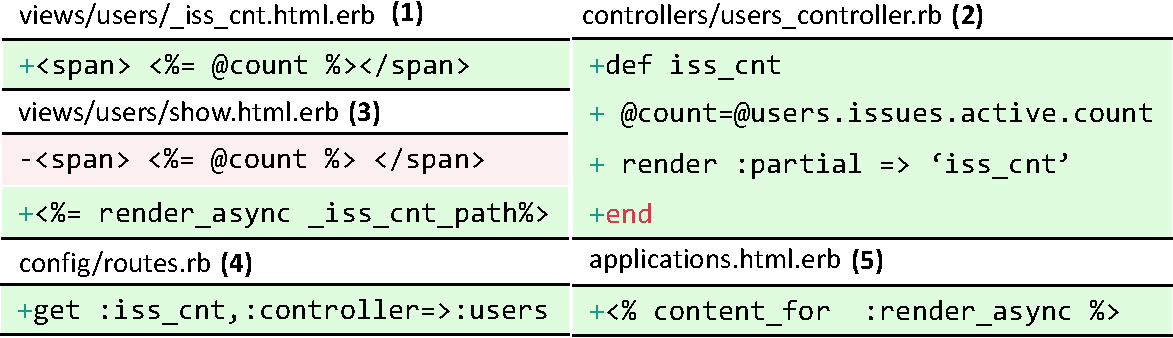
\includegraphics[width=\columnwidth]{panorama-figs/async.pdf}
    \caption{Refactoring for asynchronous loading}
    \label{fig:async}
     \vspace{-0.2in}
\end{figure}

The first item is straight-forward to automate.
\Tool simply moves the HTML tag $e$ into a newly created view file,
like {\tt \_iss\_cnt.html.erb} (Figure \ref{fig:async}(1)), where {\tt iss\_cnt} corresponds to the 
name of the new controller action that \Tool will generate. 



The second item 
%is non-trivial
%and could be error-prone for developers
%to carry out manually. 
is implemented by \Tool in three steps.
It first identifies all Ruby variables
used by $e$, like {\tt @count} in Figure \ref{fig:async}(1), and then
applies static backward slicing to find all code statements $C$
that are used to compute those variables, like
{\tt @count = @user.issues.active.count} in Figure \ref{fig:async}.
Specifically, \Tool starts from all the ADG nodes associated with
the specific HTML-tag ID, and traces backwards in the ADG to identify all nodes inside the corresponding
controller that $e$ has control or data dependence on.

\Tool next applies forward taint analysis to see if any statement $c \in C$
is used to compute any other HTML tag $e'$. If such an $e'$ is
found, there is a dilemma about whether to render $e'$ asynchronously: 
rendering $e'$ asynchronously could potentially
cause many other HTML tags, which share common backward slicing
fragments with $e'$, to be rendered asynchronously, and violate the 
design principle discussed in Section \ref{sec:async_op}; yet rendering $e'$ synchronously
incurs extra overhead as $c$ now needs to be computed twice,
%could cause server-resource wasting\cong{``server resource'' sounds strange, as resource usually means memory/bandwidth/..., and I think here it means server time?}, as $c$ now needs to be computed twice,
once for $e$ and once for $e'$. 
Hence, \Tool currently considers $e$ as unsuitable for asynchronous loading if $e'$ exists. 
%Of course, future extension of \Tool can be more flexible
%and introduce a threshold,
%like making no more than $K$ elements asynchronous at a time.

\Tool finally moves the slice identified earlier to a new controller action, like
{\tt iss\_cnt} in Figure \ref{fig:async}(2) (the deletion from the previous controller is not shown for simplicity), and add a rendering statement
at the end of the action,
like  {\tt render :partial => `iss\_cnt'} in Figure \ref{fig:async}(2),
to render the same content
in the same format as the original web application using the newly created view file.

\Tool conducts the third item leveraging the {\tt render\_sync} library \cite{asyncgem} to replace the original HTML tag with 
``{\tt<\%= render\_async [action]}
{\tt \_path \%>}'' (Figure \ref{fig:async}(3)), where {\tt render\_async}
is an API call that issues an AJAX request for the specified
{\tt action} using jQuery~\cite{jquery}.
\Tool then adds a new rule into the routing file
to connect the AJAX request with the action it just created.
As shown in  
Figure \ref{fig:async}(4), this new routing rule follows the template
``{\tt get :[action], :controller =$>$} {\tt :[home]}'', 
where {\tt action} is the name of new action name, and 
{\tt home} is the controller holding the {\tt action}.


\subsection{Display-accuracy change: approximation}
\label{sec:approx}

\begin{figure}
    \centering
    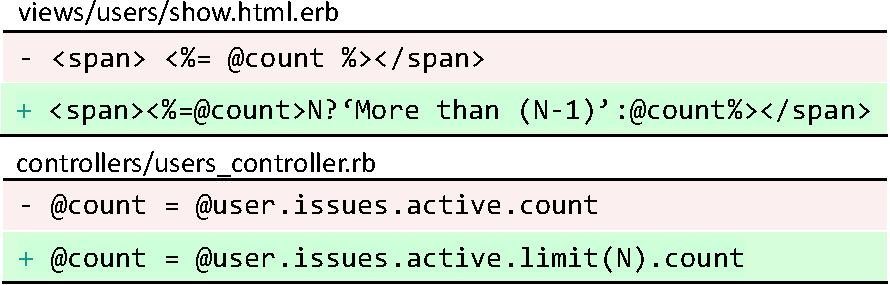
\includegraphics[width=\columnwidth]{panorama-figs/approxi.pdf}
    \caption{Refactoring for approximation}
    \label{fig:approxi}
    \vspace{-0.2in}
\end{figure}

Approximation is a widely used approach to improving performance and saving server resources \cite{farrell2016meantime}. 
Past database research also proposed approximated
queries \cite{motwani:cidr03:query}. However, many techniques require 
changes to database engines \cite{ioannidis:vldb99:histogram} and hence
cannot be applied to web application refactoring. \Tool focuses on approximating
aggregation queries whose results are displayed as numeric values on web pages,
as such approximation can be simply conducted by refactoring Rails code
and easily reasoned about by web viewers.

For example, 
Redmine \cite{redmine} is a project collaboration application like GitHub. Its  {\tt user/index} page
lists all the recent activities of a user, all projects a user is involved in (with pagination), 
as well as two 
counts showing how many issues are currently assigned to and have been reported by 
this user.
%, as shown in Figure~\ref{fig:redmine}. 
Although these two numerical counts occupy tiny space on the web page,
they can take more time, even more than 1 second, to render than the remaining page,
when a user is involved in hundreds of or more issues. 
One way to keep the page responsive is to set an upper-bound to such a count, like $100$, and only
shows the count to be ``{\it more than 100}'' when it is too big --- when a count is too big,
 users probably does not care about the exact number anyway.

\iffalse
\begin{figure}
    \centering
    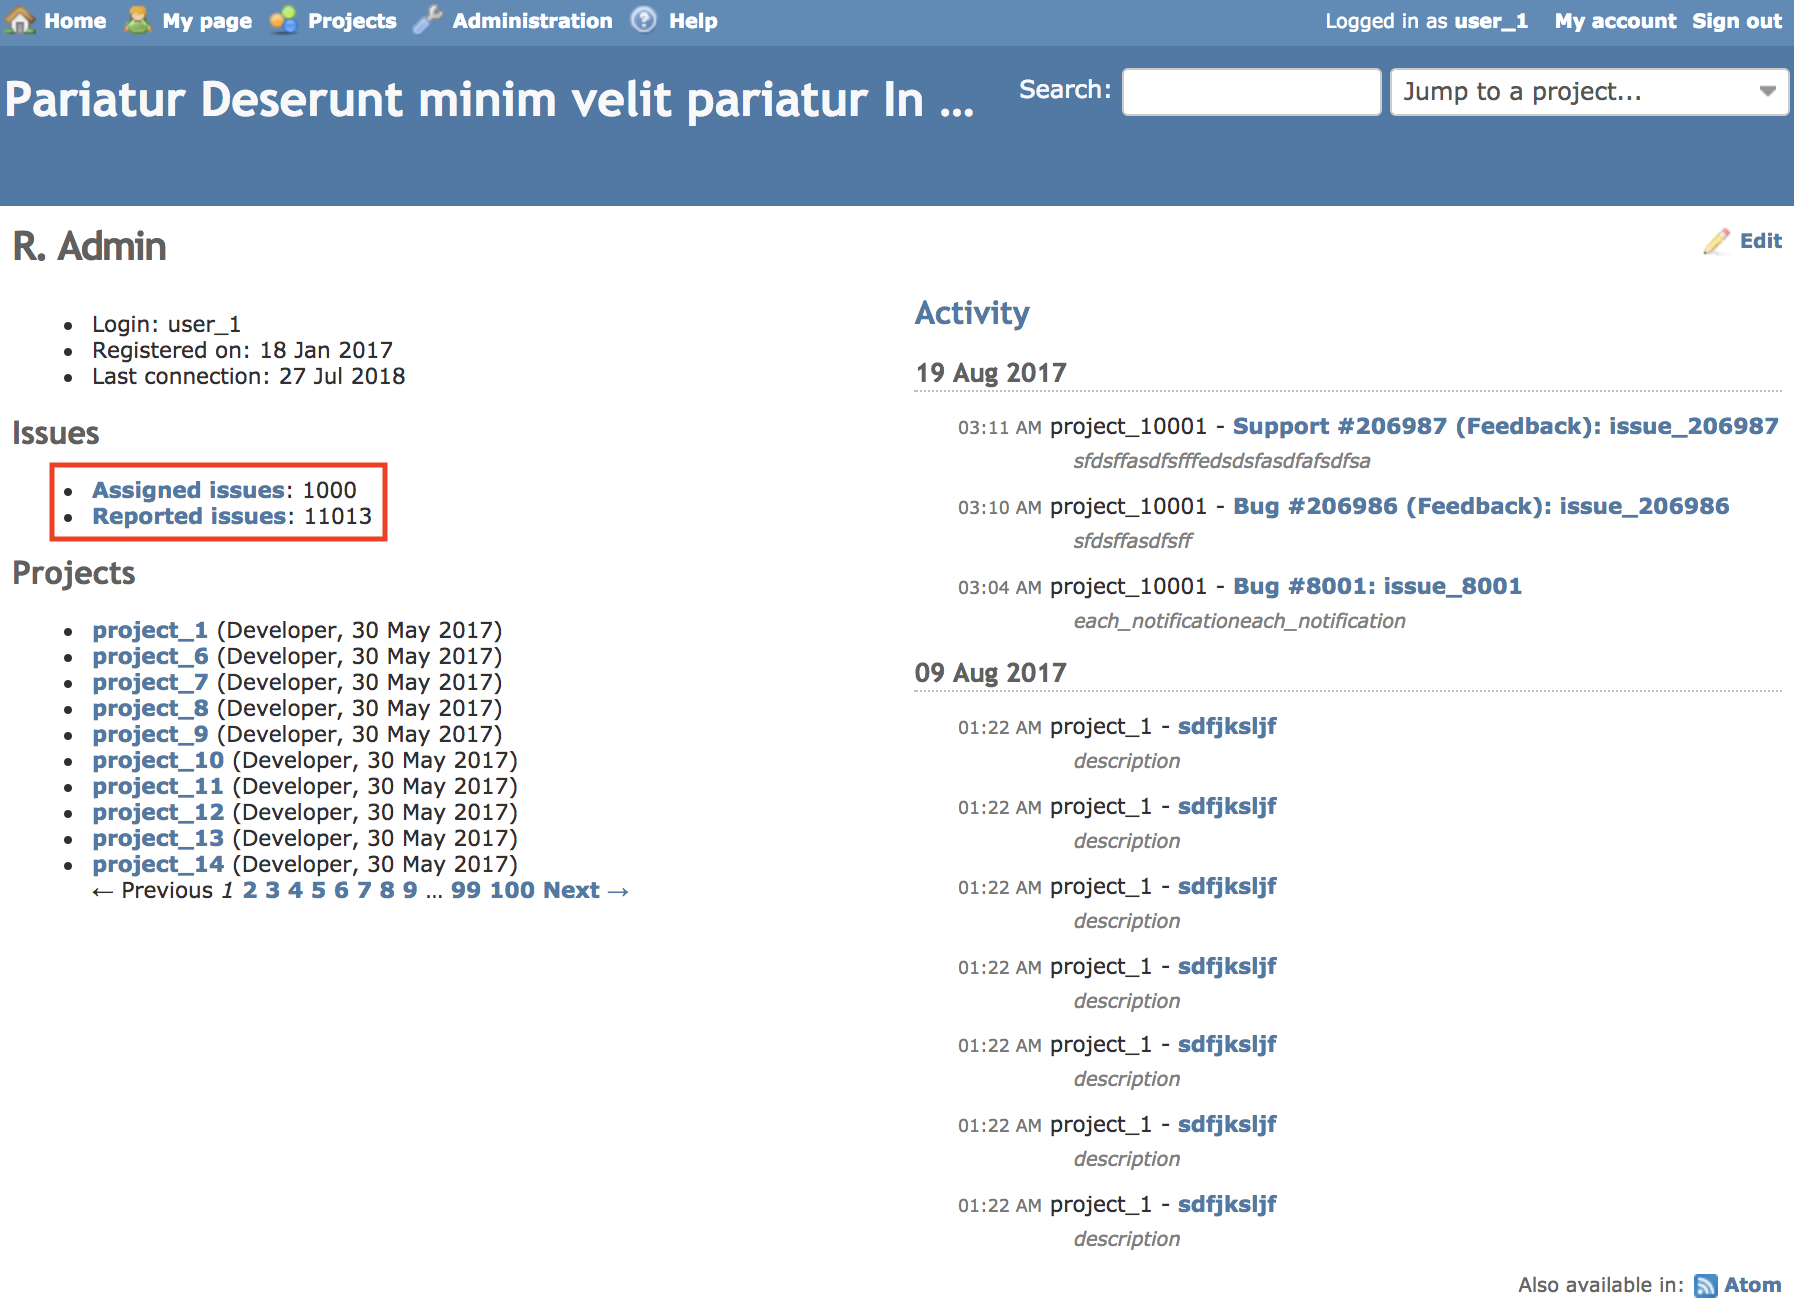
\includegraphics[width=\columnwidth]{figs/redmine.png}
    \caption{Redmine users/1 page}
    \label{fig:redmine}
\end{figure}
\fi

\subsubsection{Identifying opportunities}
\Tool iterates through all aggregation, including
maximum, minimum, average, and count,
queries in the application. 
For each query, \Tool checks its corresponding ADG node's
out-going data-flow edges to
see if the query result is {\it only} used in
HTML-tag rendering. 
If so, an approximation opportunity is
identified for corresponding HTML tag(s). 
Note that, \Tool does not suggest approximating an aggregation query if its result affects
an HTML tag through control dependency, as that type of approximation may
cause program execution to take a different path and hence potentially leads
to large deviation from original program behaviors. 
%\cong{why?}\shan{err, I revised a little bit.
%is it clear now?}\cong{yes}

\subsubsection{Generating patches}
An approximation refactoring includes two parts. 
On the controller side, \Tool appends a {\tt limit(N)} clause to the end of the
aggregation query identified above, with the constant $N$ configured by 
web developers. On the view side, instead of directly displaying the
numeric query result, changes are made depending on the aggregation query type.
For a {\tt count} query, \Tool inserts a conditional statement to check the aggregation result: if the result is smaller than $N$ then the accurate numerical result is displayed, otherwise
``more than $N-1$'', as shown in Figure \ref{fig:approxi};
for an average query, \Tool adds ``{\tt about}'' before the numeric query
result rendered in the HTML tag; for a maximum or minimum query,
\Tool adds ``{\tt at least}'' or ``{\tt at most}'' before the numeric query
result.



\subsection{Display contents removal}

Obviously, one can remove an HTML tag to speed up the page loading. 
This strategy is indeed used in practice, as the {\tt Tracks} example discussed in
Section \ref{sec:intro}.
Whether an HTML tag is worthwhile to display cannot be determined automatically.
Instead, what \Tool can do is to make the removal easy and error-free, so that developers
can easily try out different design options and eventually make an informed decision.

% \iffalse
% For example, a popular task-management application Tracks \cite{tracks} has a
% %{\tt todos/index} page. The {\tt todos/index} page mainly 
% page that lists the todos in the left pane. This page %and it 
% has a right sidebar to retrieve and display all the projects and contexts of the
% current user, which takes a lot of time for user who takes part in large number of projects. In the side-bar code, the only data-related \cong{data-related?} part
% is simply a {\tt @sidebar.active\_projects} and a {\tt @sidebar.active\_contexts} statement, which seem
% like \cong{why mention ``seem like...'' and why mention these two statements (I assume they are function calls but you do not explain what's in the function)?} a trivial heap access but actually issue a {\tt SELECT} query and
% retrieves the projects and contexts. Later on in tracks-870, the developers made a trade-off between performance
% and functionality by deleting the sidebar completely,
% %and not showing users the projects and contexts. 
% \shan{how many? how can a user be involved in many projects? What is the expensive query behind} \junwen{The complain says he has 80 projects which will grow pu to 150 projects later on}
% %to render. Eventually, developers decided to delete this side-bar completely, %which 
% providing xxx speed-up to this web page. 
% \fi
 
\subsubsection{Identifying opportunities}
Removing an HTML tag $e$ does not guarantee to save page-loading time, because if the expensive
computation needed by $e$ is also needed by other HTML tags, removing $e$ alone will not help
performance much. The current prototype of \Tool only suggests removing an HTML tag $e$ if its contributing query that is not fed to any other HTML tag.
%\cong{if so, how do you remove a sidebar that contains many elements?}
%\shan{currently, we just don't unless those items are displayed inside one HTML tag}. 
This way, removing $e$ can guarantee to save some data-processing time.
Of course, future work can relax this checking criterion.
\begin{figure}
    \centering
    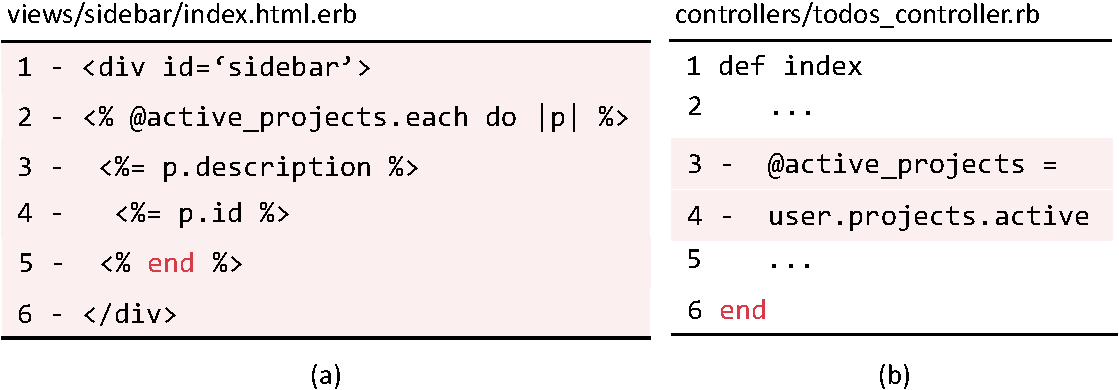
\includegraphics[width=1\columnwidth]{panorama-figs/remove.pdf}

    \caption{code change for removing}
    \label{fig:remove}
    \vspace{-0.2in}
\end{figure}

\subsubsection{Generating patches}
Removing an HTML tag $e$ from the web page again involves changes to both the
view component and the controller component of a web application.
On the view side, \Tool simply removes the specific HTML tag.
On the controller side, \Tool again analyzes control-dependency and data-dependency graph
to remove code that was used only to help generate $e$.

To do so, \Tool first identifies all the nodes in ADG that are associated with $e$'s ID.
\Tool deletes those nodes, removes all condition checking whose two branches
now execute exactly the same code because of those node deletions, and then 
check if there are any other ADG nodes that
become useless and should be deleted
--- a node is useless if it has no out-going data-dependency or control-dependency
edges. \Tool repeats
this process for several rounds until no more nodes are identified as useless. 

We use the view file code snippet in Figure \ref{fig:remove}a as an example.
The HTML tag shown here corresponds to the sidebar
that lists all projects 
in the Tracks example discussed in 
Figure \ref{fig:crossstack}.
%, as shown in Figure\ref{fig:heatmap}
Given this tag, \Tool first identifies the
Ruby expression {\tt @active\_projects}, and then checks the ADG to see how 
{\tt @active\_projects} is computed in the
controller (Figure \ref{fig:remove}b).
\Tool also finds out that the 
{\tt @active\_projects} computed in 
Figure \ref{fig:remove}b is not used in anywhere
else.
%\shan{What is
%show-guidelines? Is this a function or what?}, and
Consequently, the content-removal change will simply
delete the sidebar tag in the view file
%computing statement
and the corresponding computation
in the controller file, as shown in 
Figure \ref{fig:remove}.


%\shan{can we extend this to removing the condition checking of a HTML element display?}

%\iffalse

%\fi